\documentclass{article}
\usepackage{makeidx}
\usepackage{graphicx}
\usepackage{titlesec}
\setcounter{secnumdepth}{4}
\usepackage[utf8]{inputenc}

\title{mycc - My own C++ compiler implementation}
\author{Hanze Chen}
\date{January 2022}
\makeindex

\begin{document}
\maketitle
\section{Introduction}
    \begin{figure}[hb!]
        \centering
        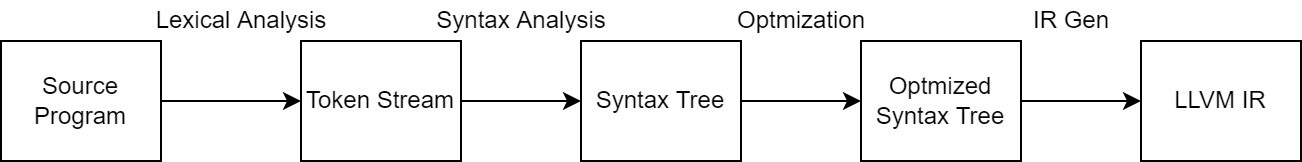
\includegraphics[width=10cm]{figure/frontend_structure.png}
        \caption{Frontend Structure}
        \label{Fig:frontend_structure}
    \end{figure}
\section{Implemented Function}
\subsection{Part0}
    When part 0 is enabled by "-0" option. The compiler will only generate the output like Figure \ref{Fig:example_part0_output} Shows: \par
    \begin{figure}[hb!]
        \centering
        \fbox{
            \shortstack[l]{
                My bare-bones C compiler (for COM 440/540) \\
                Written by Hanze Chen (hanzech@iastate.edu) \\
                Version 0.1.0\_9c370c3(WorkStation) \\
                2022-01-28 13:18:14
            }
        }
        \caption{Example Output for Part 0}
        \label{Fig:example_part0_output}
    \end{figure}

    Version string is in format of Major\_Minor\_Patch\_Commit Hash(compile machine's hostname). And the last line is the build time. In my implantation those variables will generate when CMake projects is finished its configuration step. And those variable will be run-time accessible via “version.h" which will generate by CMake from "version.h.in" \par

    When compiler is running in part 0 mode (with "-0" flag), the compiler will not processing any input file, and will always write the version message like Figure \ref{Fig:example_part0_output} to output file (declared by "-o" flag)
\section{Main Data Structures}
    \subsection{Lexical}
        \subsubsection{LexicalToken \index{Lexical Token Class}}
            Recall the compiler frontend workflow described in Figure \ref{Fig:frontend_structure}. TokenStream is defined as a list of LexicalToken class which contains all parsed available token in source file.\par
            Currently all the supported lexical token type and its regex expression is included in Table \ref{table:supported_lexical_token_list}: \par
            \begin{table}[hb!]
                \centering
                \begin{tabular}{l|lll}
                    \hline
                    Token Type  & Regex                                                  & Example           & Description    \\ \hline
                    add         & \textbackslash{}\textbackslash{}+                      & +                 & Addition       \\
                    sub         & -                                                      & -                 & Subtraction    \\
                    mul         & \textbackslash{}\textbackslash{}*                      & *                 & Multiplication \\
                    div         & /                                                      & /                 & Division       \\
                    number      & {[}0-9{]}+\textbackslash{}\textbackslash{}.?{[}0-9{]}* & 0, 0.1 etc.       & Numbers        \\
                    Identifiers & {[}a-zA-Z\_{]}{[}a-zA-Z0-9\_{]}*                       & "a", "while" etc. & Identifiers    \\ \hline
                \end{tabular}
                \caption{Supported Token Type}
                \label{table:supported_lexical_token_list}
            \end{table}
    \subsection{Utils}
        \subsubsection{Status \index{Status Class}}
\section{User Manual}

\printindex
\end{document}
